%%==================================================
%% chapter01.tex for SJTU Master Thesis
%%==================================================

\chapter{Introduction}

\section{Motivation}
% motivation
With the spread of mobile devices, our life are crowded with many multimedia resources. 
Today, hundreds of millions pictures are being take, videos are uploaded, and a large amount of audio clips are also being recorded. 
Among these multimedia resources, audio data often contains many useful information around the device. 
For example, in an audio recorded under the context of office, we may hear "computer keyboard typing" and "phone ringing", sometimes with "people talking" as the background sound. 
After hearing these sound features, we human could easily deduce that the clips we heard are recorded in an office-like context. 
But this scene recognition process could be further speed up or applied to large quantity audios by a automatically scene recognition system.  

The automatical recognition for audio scenes are important for audio content analysis. 
For example, in the modern life, people tend to carry their mobile phones everywhere with them. 
It would be more convinient if the mobile devices could automatically adjust their volume and other profile settings according to the surrounding environment. 
This may prevent the trouble of unexpected loud noise by mobile devices in an quiet scene, or could save us from missing important notifications when we are surrounded by noisy atmosphere.  
Moreover, this technique not only could be applied in ordinary conditions, but also in some security issues. 
In the surveillance process, police may receive hundreds of thousands videos and audio clips. 
The automatic scene recognition technique may help to them fast analyze those audios and pindown the scenes they want to further analyze. 

\section{Problem Description}
Figure \ref{fig:waveform} shows an example waveform for a concert environment. 
In this clip, two things happened. 
The first part of this waveform represents the sound when people are applauding. 
The second part is the sound when musicians are tuning their instruments. 
For a human, upon hearing these two things, we are easily to tell that this audio is recorded in a concert. 
And our problem throughout this thesis is to automatically detect out the events like \textit{applause} and \textit{instrument tuning}, 
and then to infer the scene \textit{concert} based on these two detected events. 

\begin{figure}[htb]
\centering
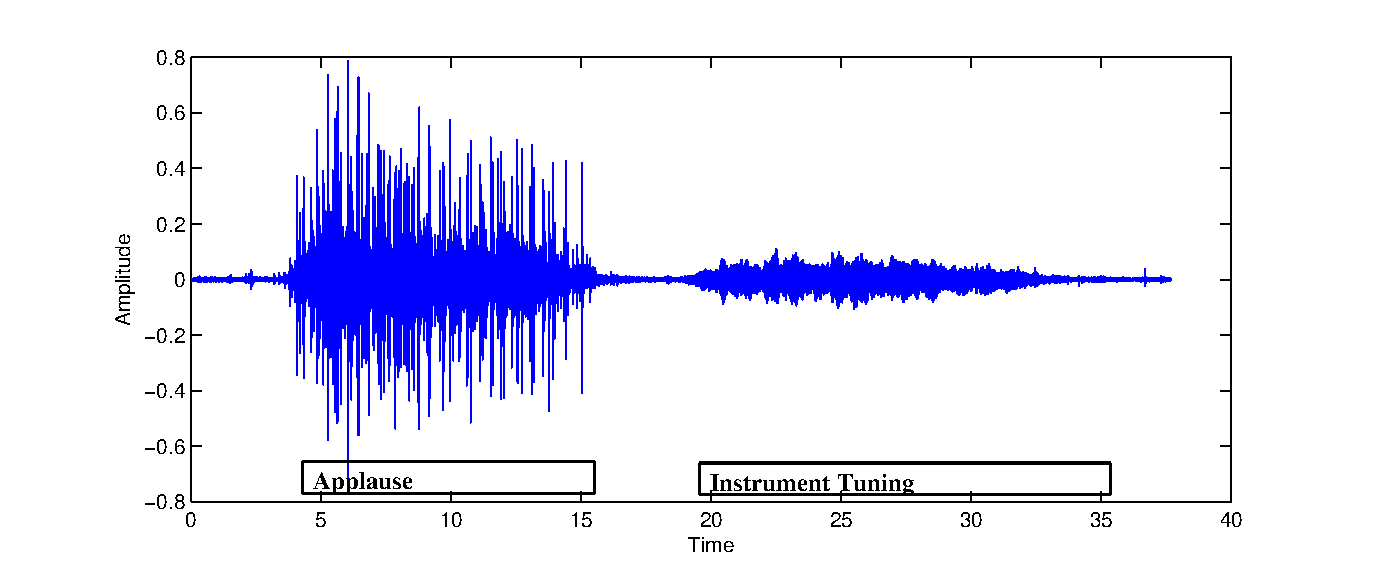
\includegraphics[scale=0.6]{figure/intro/waveform}
\caption{Waveform for a concert audio clip}
\label{fig:waveform}
\end{figure}

At here, we would like to give a detailed definition some terminology that we are going to use in this thesis. 
First, the term \textit{audio scene}, or \textit{audio context} is used to as the name for a comparatively isolated sound environment. 
The word \textit{isolated} here means that different scenes could be distinguish by human from the audios.  
\textit{Office}, \textit{subway station}, and \textit{restaurant} are some common indoor audio scenes. 
While \textit{forest}, \textit{street}, and \textit{park} are some common outdoor audio scenes. 
In another way, the scene could be the name we used to describe some places, where some sound may be heard under those places. 
 
Audio scene is a broad acoustic concept, and apart from it, we have used another term called \textit{audible events}. 
Events originally means a thing, and audible events here means an item or a movement that usually has a sound associated with it. 
Like, we consider \textit{car honk}, \textit{phone ring}, and \textit{footstep}, etc., as audible events. 
The difference between audible events and audio scenes lies in the granularity of a concept. 
Audible events generally represent more specific sounds, and are constituents in audio scenes. 
Audio scenes include some audible events, they represents the overall atmosphere. 
We could say in a sense that audio scenes are comprised of audible events. 

So the problem that we want to solve in this thesis is to detect audible events in a clip, and then infer the audio scenes the original clip is in. 

\section{Our Approach}
So in this thesis, we have proposed a system to automatically detect the events in an audio clip and then infer the scene or context from the detected audio events. 
For audible events, we constructed an audible event taxonomy, which helps us to categorize common audible events. 
This taxonomy we created groups different audible event by their characteristics. 
For example, \textit{car}, \textit{train}, \textit{subway} are all grouped into the category of \textit{transport}. 
Building such a taxonomy helps us organize our audible events, instead making an arbitrary list to include all the possible sounds. 
Then for all the audible event candidates, we query them in the search engine of some websites that host a collection of audio sounds. 
We download all the clips returned by the sound search engine that satisfies a duration condition, i.e., we discard sound which are either too short or too long, since they may not be a valid clip for our audible events.  

Feature extraction for the downloaded audio clips are carried out using Mel-Frequency Cepstrum Coefficients (MFCCs). 
It is a popular feature for speech recognition, and we use it in our problem for the event feature extraction. 
Then Gaussian Mixture Models (GMMs) are built for modeling these features. 
We choose GMMs to model these data because of their speed and the dynamic number of components. 
The sound for an audible event may contain several parts. 
Different gaussian components could be used to model various parts and form a model representing the audible event. 

In the scene recognition process, we first segment an audio clip by a segmenter, which uses frame energy and spectral centroid to calculate a threshold. 
After detecting for these segments, we utilize the relation we found in movie, play and TV series scripts. 
Because those scripts come with different scenes already specified in it, we could use that information to analyze the paragraphs under a known scene name. 
This analysis process is conducted by calculating a TF-IDF score of audible events to scenes. 
This score measures the importance of a event to a scene, thus can be used a suitable score when we are inferring scenes. 

\begin{figure}[htb!]
\centering
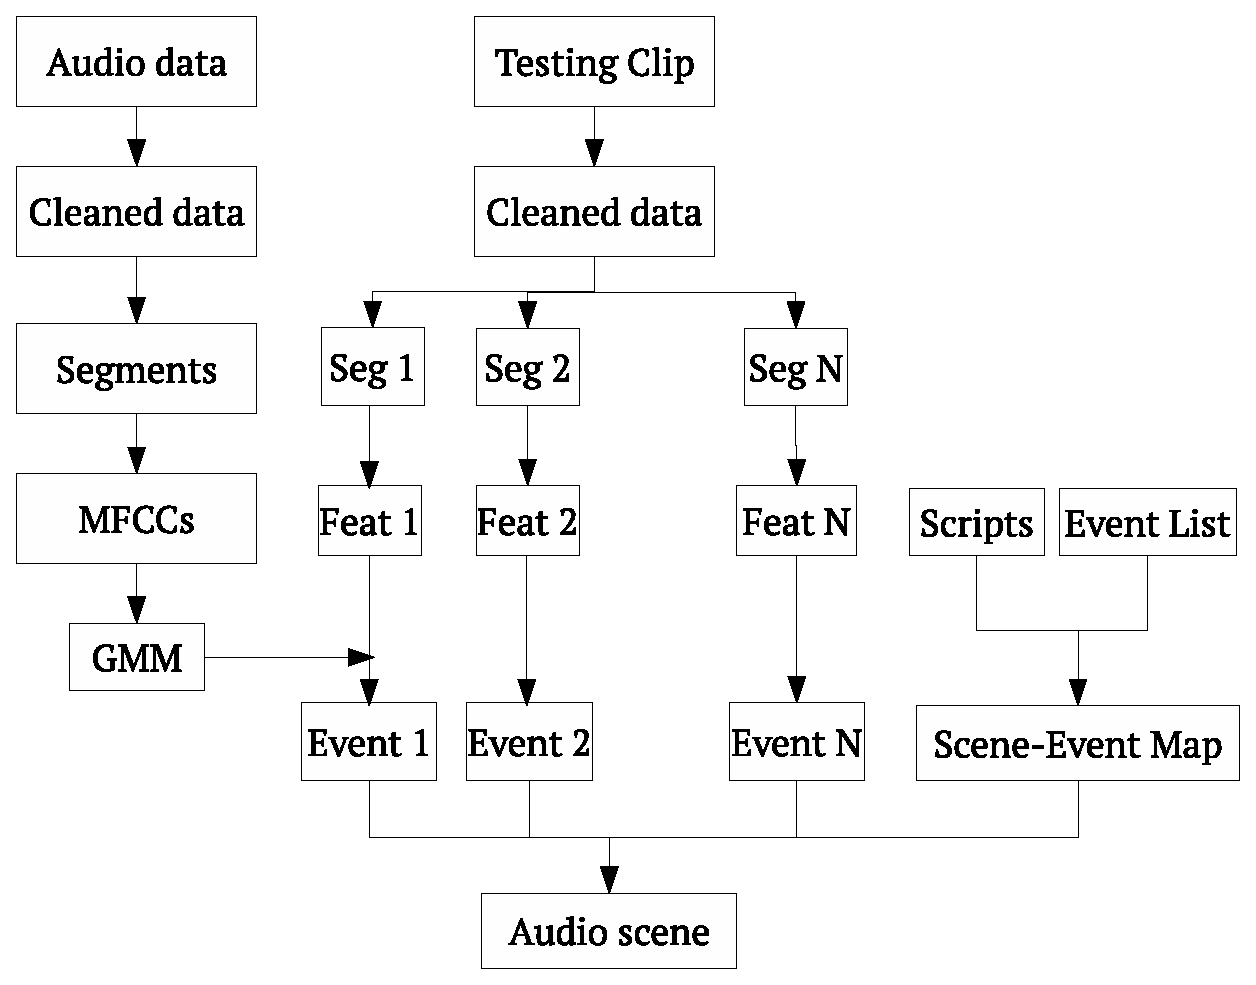
\includegraphics[scale=0.6]{figure/intro/structure}
\caption{Design of our scene recognition system}
\label{fig:structure}
\end{figure}

Figure \ref{fig:structure} shows the overall structure of this project. 
The structure can be viewed as three parts. 
The left part describes the training process, i.e., downloading data, preprocessing clips, segments, feature extraction, and model training. 
The right part is the process of constructing scene-event relation map by the knowledge of movie, play and TV series scripts and event list from our taxonomy. 
Presented in the middle is our testing part. 
Whenever a testing clip is presented, it goes through the same preprocessing, segmentation step. 
Then each segments are individually detected by our pretrained GMMs, thus yield an event label for each segments. 
Combining the scene-event map with the sequency of detected audible events, we use a voting mechanism to select out the most likely audio scene of the original testing clip. 

\section{Thesis Organization}
The thesis is organizaed as follows: Chapter 2 gives a description about related works, in the area of audible events taxonomy, audio event detection and audio scene recognition. 
Chapter 3 reviews the data we used in this thesis, including event list and scene list. 
The process of creating the audible event taxonomy is introduced, and we describe the way we use our script data to crawl scene names. 
Then in chapter 4 we describes how event detection is carried out, including feature extraction, model training, etc. 
Chapter 5 present the method we used to extract scene-event relations and scene recognition process. 
The calculation of a TF-IDF score is discussed in detail, and a segmenter algorithm is introduced. 
Evaluations of event detection and scene recognition are presented in chapter 6, where both include a self tuning evaluation and a model comparison. 
Finally, chapter 7 gives a conclusion and analyze our current deficience.   
Some directions for future work are also given. 

